%!TEX root = ../rapport.tex
%!TEX encoding = UTF-8 Unicode

% Chapitres "Introduction"

% modifié par Francis Valois, Université Laval
% 31/01/2011 - version 1.0 - Création du document

\chapter{Diagrammes de séquences}
\label{s:sequences}
Ce chapitre présente les différentes figures associées au diagramme des séquences. Ce diagramme est séparé selon cinq portions relatives aux fonctions particulières du robot. La figure \ref{fig:diagSeq1Ite1} présente les liens entre l'utilisateur et la kinocto. La figure \ref{diagSeq2Ite1} présente les liens entre la kinocto et son environnement afin de déterminer sa position. La figure \ref{diagSeq3Ite1} présente les liens entre la kinocto et la station de base pour la transmission et l'affichage de la trajectoire optimale.La figure \ref{diagSeq4Ite1} présente les liens entre la kinocto et la table de jeu dans l'optique du déplacement de celle-ci à travers les obstacles vers la zone de lecture ainsi que les liens avec la résolution du sudocube. La figure \ref{diagSeq5Ite1} présente les liens entre la kinocto et ses différents périphériques lors de la production du dessin et de la confirmation de la résolution de la tâche.
\begin{figure}[htb]
\centering
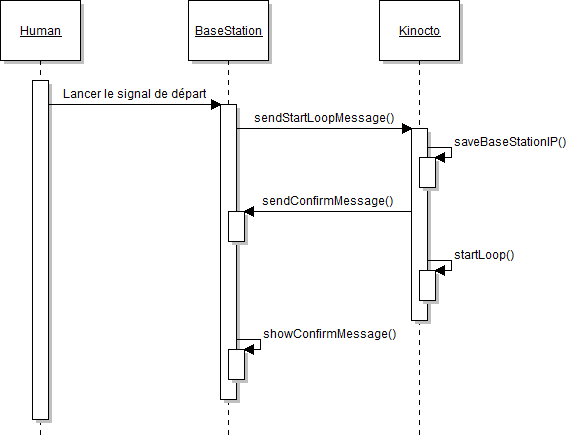
\includegraphics[scale=0.75]{diagSeq1Ite1.png}
\caption{Diagramme des séquences présentant les liens entre l'utilisateur et la kinocto}
\label{fig:diagSeq1Ite1} 
\end{figure}
\begin{figure}[htb]
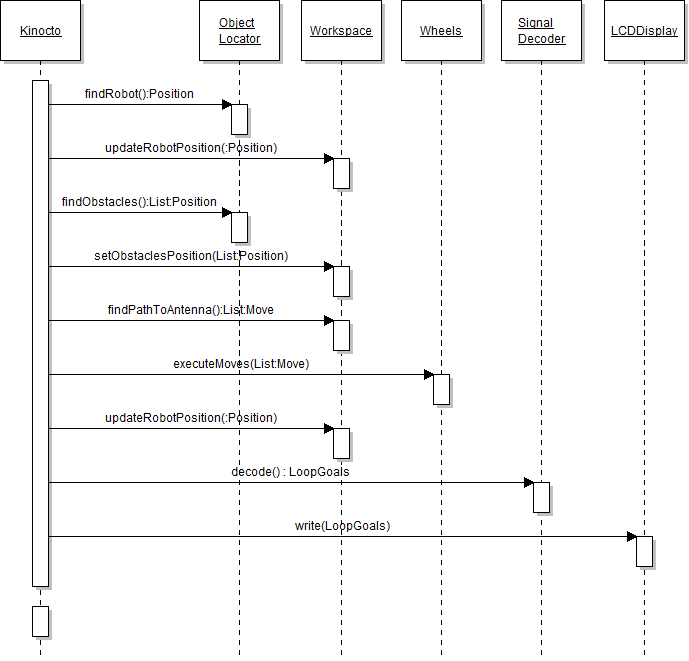
\includegraphics[scale=0.65]{diagSeq2Ite1.png}
\caption{Diagramme des séquences présentant les liens entre la kinocto et son environnement afin de déterminer sa position}
\label{diagSeq2Ite1}
\end{figure}
\begin{figure}[htb]
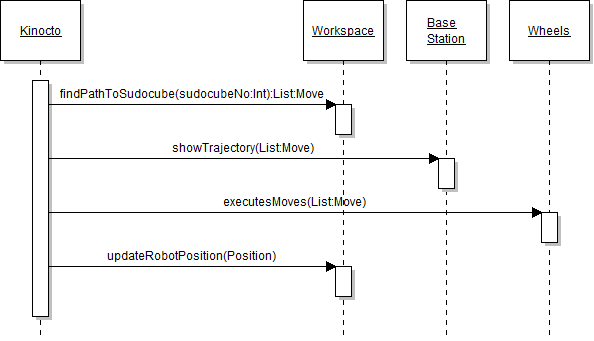
\includegraphics[scale=0.75]{diagSeq3Ite1.png}
\caption{Diagramme des séquences présentant les liens entre la kinocto et la station de base pour la transmission et l'affichage de la trajectoire optimale}
\label{diagSeq3Ite1}
\end{figure}
\begin{figure}[htb]
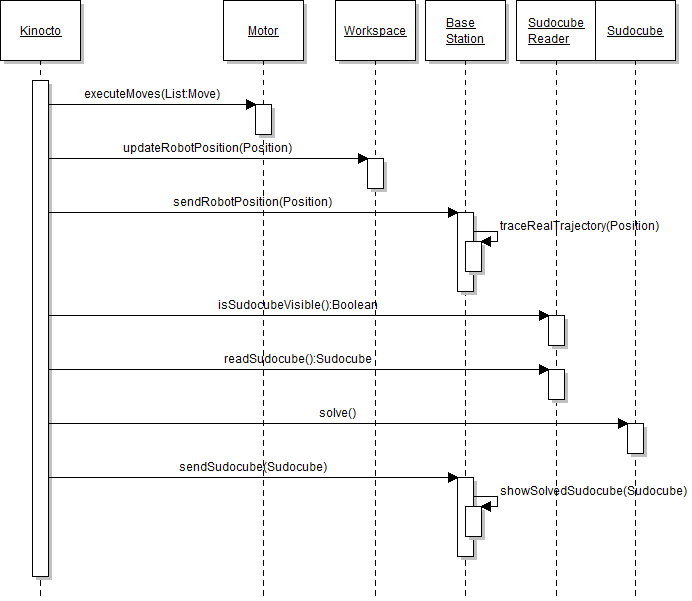
\includegraphics[scale=0.65]{diagSeq4Ite1.png}
\caption{Diagramme des séquences présentant les liens entre la kinocto et la table de jeu dans l'optique du déplacement de celle-ci à travers les obstacles vers la zone de lecture ainsi que les liens avec la résolution du sudocube}
\label{diagSeq4Ite1}
\end{figure}
\begin{figure}[htb]
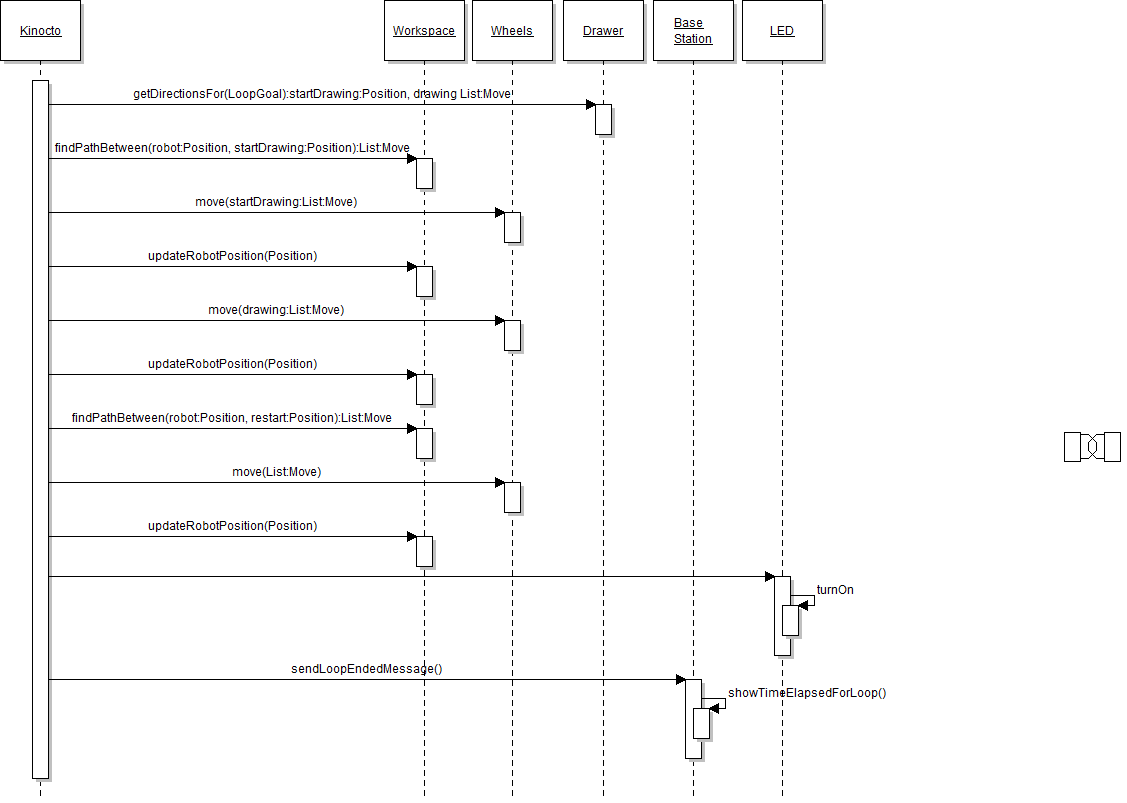
\includegraphics[scale=0.5]{diagSeq5Ite1.png}
\caption{Diagramme des séquences présentant les liens entre la kinocto et ses différents périphériques lors de la production du dessin et de la confirmation de la résolution de la tâche}
\label{diagSeq5Ite1}
\end{figure}
